\documentclass[
  a4paper,            % DIN A4
  DIV=10,             % Schriftgröße und Satzspiegel
  oneside,            % einseitiger Druck
  BCOR=5mm,           % Bindungskorrektur
  parskip=half,       % Halber Abstand zwischen Absätzen
  numbers=noenddot    % Kein Punkt hinter Kapitelnummern
]{scrreprt}
\usepackage{../style/thesisstyle}

\newcommand\note[1]{\textcolor{red}{#1}} % text within the \note command will be red (implicating a TODO)

\makeglossaries           % create all glossary entries (remember: run makeglossaries manually)
\loadglsentries{thesisglossaries.tex}  % load acronym, symbol and glossarie entries

\begin{document}
% !TEX root = ../thesis.tex
%
% configurations
%

% text field
%-> replace supervisor names with correct ones
\firstSupervisor{Prof. Dr.-Ing. Andreas Meisel}
\secondSupervisor{Prof. Dr. rer.nat. Stephan Pareigis}

% text field
%-> replace title with your thesis title
\thesisTitle{Bildbasierte Navigation mit Neuronalen Netzen}
\thesisTitleEN{Image based navigation with Neural Networks}

% text field
%-> replace the key words with your own key words
\keywordsDE{Leben, Universum, Alles}
\keywordsEN{Life, Universe, Everything}

% text field
%-> replace the text with a description of the thesis
\abstractDE{In dieser Bachelorarbeit soll untersucht werden, wie Navigation auf reinen Bildaten funktionieren kann. Konkret geht es um das Erkennen einer Fahrbahn mit einem Neuronalen Netz, bzw. um das Erzeugen von Lenkwinkeldaten auf Basis eines Bildes einer Fahrbahn. Hierzu wird ein trainiertes Neuronales Netz mittels Fine Tuning abgestimmt.  Das wid direkt zur Anwendung gebracht auf einem RC Fahrzeug aus dem "Carolo-Cup", inklusive Fahrten auf einer Teststrecke. }
\abstractEN{Arthur Dents travel to a new future \dots}

% text field
%-> replace jon with your name
\thesisAuthor{Jan Robert Rösler}

% text field
%-> enter the submission date
\submissionDate{07. Juni 1954}

% switch - uncomment only one
%-> uncomment NDA or public
%\NDA{yes}
\NDA{no}

% switch - uncomment only one
%-> uncomment to show list of figures or not 
\ListOfFigures{yes}
%\ListOfFigures{no}

% switch - uncomment only one
%-> uncomment to show list of tables or not 
\ListOfTables{yes}
%\ListOfTables{no}

% switch - uncomment only one
%-> uncomment to show list of accronyms or not 
\ListOfAccronyms{yes}
%\ListOfAccronyms{no}

% switch - uncomment only one
%-> uncomment to show list of symbols or not 
\ListOfSymbols{yes}
%\ListOfSymbols{no}

% switch - uncomment only one
%-> uncomment to show list of glossary entries or not 
\Glossary{yes}
%\Glossary{no}

% switch - uncomment only one
%-> uncomment the study course you are in
%\studycourse{ITS}
\studycourse{TI}
%\studycourse{AI}
%\studycourse{WI}
%\studycourse{EI}
%\studycourse{BMT}
%\studycourse{MAI}
%\studycourse{MIK}
%\studycourse{MA}
    % load all settings

\hyphenation{Ba-che-lor-the-sis Mas-ter-the-sis}

% Cover page here, no page number
% !TEX root = ../thesis.tex
%
% cover page
% @author Thomas Lehmann
%

\thispagestyle{empty}
\begin{titlepage}
{\fontfamily{phv}\selectfont

% NDA, if needed
  \hfuzz=20pt
\begin{textblock*}{\textwidth}(75mm,9mm)
  \begin{minipage}[b][0cm][b]{\textwidth}
  \hfuzz=20pt
  \fontsize{16pt}{16pt}
  \selectfont
    \begin{flushleft}
    	  \IthesisNDAFull
    \end{flushleft}
  \end{minipage}
\end{textblock*}

% black-white logo
\begin{textblock*}{\textwidth}(134mm,40mm)
  \begin{minipage}[b][0cm][b]{\textwidth}
    
\includegraphics[scale=0.5]{../style/HAW_Marke_schwarz}
  \end{minipage}
\end{textblock*}

% kind of thesis
\begin{textblock*}{\textwidth}(30mm,115mm)
  \begin{minipage}[b][0cm][b]{\textwidth}
    \fontsize{22pt}{20pt}
    \selectfont
  	\begin{flushright}
      \IthesisKind
  	\end{flushright}
  \end{minipage}
\end{textblock*}

% author of thesis
\begin{textblock*}{\textwidth}(30mm,140mm)
  \begin{minipage}[b][0cm][b]{\textwidth}
  \fontsize{14pt}{20pt}
  \selectfont
    \begin{flushright}
      \IthesisAuthor
  	\end{flushright}
  \end{minipage}
\end{textblock*}

% Title of thesis
\begin{textblock*}{\textwidth}(30mm,155mm)
  \begin{minipage}[b][0cm][t]{\textwidth}
  %\fontsize{18pt}{20pt}
  \ITitleFontSize
  \selectfont
  	\begin{flushright}
       \IthesisTitle
  	\end{flushright}
  \end{minipage}
\end{textblock*}

\ITextBlockSupervisionOnCover

% german version of faculty and department
\begin{textblock*}{\textwidth}(20mm,256mm)
  \begin{minipage}[b][0cm][t]{\textwidth}
  \fontsize{11pt}{10pt}
  \selectfont
    \begin{flushleft}
      \textit{\IthesisFacultyFull} \\
      \textit{\IthesisDepartmentFull}
    \end{flushleft}
  \end{minipage}
\end{textblock*}

% english version of faculty and department
\begin{textblock*}{\textwidth}(52mm,256mm)
  \begin{minipage}[b][0cm][t]{\textwidth}
  \fontsize{11pt}{10pt}
  \selectfont
    \begin{flushright}
      \textit{\IthesisFacultyFullEN} \\
      \textit{\IthesisDepartmentFullEN}
    \end{flushright}
  \end{minipage}
\end{textblock*}
}
\end{titlepage}
\                % this backslash is needed, otherwise LaTeX does wired things ....


% Titlepage is page one even if the number is not shown.
\pagenumbering{roman}
% Title page here
% !TEX root = ../thesis.tex
%
% title page
% @author Thomas Lehmann
% Hints for titel page and page numbering: https://en.wikipedia.org/wiki/Title_page
%
\newpage
\thispagestyle{empty}
{\fontfamily{phv}\selectfont
  \hfuzz=20pt       % suppress warnings due to extenstion onto page margins

  % Author of thesis
  \vspace*{1cm}
  \begin{minipage}[b]{\textwidth}
    \fontsize{14pt}{20pt}
    \selectfont
    \begin{center}
      \IthesisAuthor
    \end{center}
  \end{minipage}

  % Title of thesis
  \vspace{1.5cm}
  \begin{minipage}[b][0cm][t]{\textwidth}
    \fontsize{18pt}{20pt}
    \selectfont
    \begin{center}
      \IthesisTitle
    \end{center}
  \end{minipage}

  % Important information
  \begin{textblock*}{\textwidth}(40mm,210mm)
    \begin{minipage}[b]{\textwidth}
      \hbadness=10001    % suppress underfull warning due to short text
      \fontfamily{cmr}\selectfont
      \fontsize{12pt}{14pt}
      \selectfont
      \IthesisKindDE ~eingereicht im Rahmen der \IthesisExaminationDE \\
      im Studiengang \IstudyCourseName \\
      am \IthesisDepartmentFull \\
      der Fakultät Technik und Informatik\\
      der Hochschule für Angewandte Wissenschaften Hamburg\\

      Betreuender Prüfer: \IfirstSv \\
      Zweitgutachter: \IsecondSv \\

      Eingereicht am: \ISubDate \\
    \end{minipage}
  \end{textblock*}
}


% Abstract page here
% !TEX root = ../thesis.tex
%
% abstract page
% @author Thomas Lehmann
%
\newpage
\thispagestyle{plain}
\clearpage
\hfuzz=12pt       % suppress warnings due to extenstion onto page margins

\textbf{\IthesisAuthor}

\vspace{0.5cm}
\textbf{Thema der Arbeit}

\IthesisTitle

\vspace{0.3cm}
\textbf{Stichworte}

\IkeyWordsDE

\vspace{0.3cm}
\textbf{Kurzzusammenfassung}

\begin{minipage}{\textwidth}
\IabstractDE
\end{minipage}

\vspace{1.0cm}
\textbf{\IthesisAuthor}

\vspace{0.3cm}
\textbf{Title of Thesis}

\IthesisTitleEN

\vspace{0.3cm}
\textbf{Keywords}

\begin{minipage}{\textwidth}
\IkeyWordsEN
\end{minipage}

\vspace{0.3cm}
\textbf{Abstract}

\IabstractEN


% Table of contents here
\tableofcontents

% List of figures here
\IListOfFigures

% List of tables here
\IListOfTables

% List of accronyms here
\IListOfAccronyms

% List of symbols here
\IListOfSymbols

% Uncomment if list of source code is needed (rarely).
%\lstlistoflistings  % requires package listings, needs to uncommenting of usepackage

% path to the chapters folder is set to find the images used there
\graphicspath{ {./chapters/} }

% Chapters
\clearpage
\pagenumbering{arabic}
% first example chapter
% @author Jan Robert Rösler 
%


\chapter{Einleitung}


Sobald ein System, welcher Art sei offen, mobil wird, also läuft, rollt, gleitet, schwebt oder schwimmt, steht es vor der Aufgabe der Navigation. Das kann zunächst bedeuten, zu Wissen, wo es sich befindet. Auf einer Karte oder auch relativ zu anderen "Dingen"  in der Umgebung. Weiter können sich dann Fragen der Pfadplanung stellen, je nach Ziel oder Aufgabe des mobilen Systems. Ebenfalls könnte es dann von Interesse zu sein, eine eigene Repräsentation (oder Interpretation) der Umgebung aufzubauen und zu speichern, um Lokalisation und Pfadplanung kontinuierlich zu betreiben. Je nach Art und Aufgabe des Systems sind konkrete Probleme in der Navigation und ihre Lösungen zum Beispiel \note{(NAVIGATIONSPRBLEME UND LOESUNG KLASSISCH)} //


\section{Autome Navigation}




% first example chapter
% @author Jan Robert Rösler 
%
\chapter{Neuronale Navigation mit Bilddaten}

\section{Relevante Technik/Hintergrund}
Hier soll zunächst eine kurze Beschreibung der für Neuronale Navigation auf Bilddaten relevanten Technik erfolgen. Grundlegendes wird nur der Vollständigkeit halber erwähnt, speziellere Aspekte kurz vorgestellt. 

CNN 
REGRESSION


RESIDUAL (BLOCK)

LAYER FREEZING 

PreProcessing (?)

Fine Tuning 



\section{Ansätze}
Im folgenden wird auf zwei Ansätze der Navigation mit Neuronalen Netzen eingegangen, durch Gegenüberstellung erster Versuche mit einem modernen Ansatz soll folgenden Ausarbeitungen ein Rahmen gegeben werden.

\subsection{ALVINN}

Versuche durch neuronale Verarbeitung von reinen Bilddaten in einem Szenario zu navigieren, gab es bereits 1989 in Pomerleau's Arbeit, die man auf diesem Gebiet als Pionierarbeit verstehen kann.\cite{pomerleau1989alvinn}.
Das Netzwerk ALVINN (Autonomous Land Vehicle In a Neural Network) sollte das NAVLAB steuern, ein Testfahrzeug für Autonome Navigation der Carnegie Mellon University.
In \ref{img:ALVINNa} lässt sich die Architektur nachvollziehen. 
Der rein visuelle Input (die Blautstufenintensität eines Pixels bestimmt das Aktivierungslevel des Inputneurons) wird untersützt durch eine laserbasierte Abstandsmessung und ein Inputneuron für die Kodierung der \glqq Straßenintensität\grqq{}, also ob die Straße heller oder dunkler wird.
Aus heutiger Sicht ist das Netz mit nur einer hidden Layer mit 29 Neronen sehr klein, die im weiteren angesprochenen Architekturen haben deutlich mehr Layer und mehrere Hunderttausend Parameter. 
Zudem interpretiert ALVINN die Aufgabe des Spurfolgens nicht als Regressionsproblem, sondern als Klassifikation. Die Ausgangsneuronen sind eine lineare Repräsentation der Lenkrichtung, die das Fahrzeug in Richtung Fahrbahnmitte steuert. Neuronen in der Mitte stehen für eine Fahrt geradeaus, Neuronen links und rechts für die jeweilige Fahrtrichtung.
Grob gesagt gibt das Neuron mit dem höchsten Aktivierungslevel die Fahrtrichtung (den einzuschlagenden Lenkwinkel) an.
Im Ergebnis konnte das Netz nach 40 Epochen Training auf simulierten Fahrbahnbildern, zu sehen in \ref{img:ALVINNb}, einen 400 Meter Weg durch einen Wald mit \SI{1/2}{\meter/\second} sicher abfahren.//

\begin{figure}
	\centering
	\begin{subfigure}{.5\textwidth}
	\centering
		  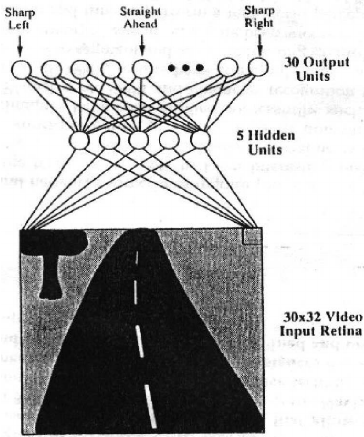
\includegraphics[width=.85\linewidth]{figures/Architecture-ALVINN.png}
		  \caption{}
		  \label{img:ALVINNa}
	\end{subfigure}%
	\begin{subfigure}{.5\textwidth}
	\centering
		  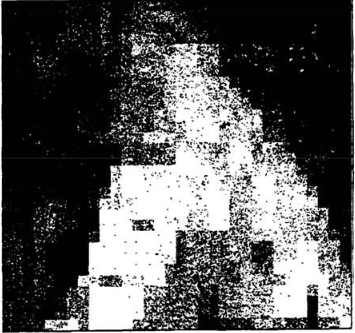
\includegraphics[width=.85\linewidth]{figures/Strasse-ALVINN.png}
	 	  \caption{}
		  \label{img:ALVINNb}
	\end{subfigure}%
	\caption{ALVINN Architektur (a) und simulierte Fahrbahn (b)}
	%Quelle: \protect\citeI{Architecture-ALVINN}
	\label{img:ALVINN}
\end{figure}

\subsection{NVIDIA DAVE-2}

Forschungserkenntnisse der folgenden Jahre trieben die Entwicklung voran und...
Im Jahr 2016 veröffentlicht das Technologieunternehmen \textsc{NVIDIA} einen eigenen Ansatz \cite{bojarski2016end}, basierend auf Versuchen mit dem \glqq DARPA Autonomous Vehicle \grqq{} (DAVE) \cite{DarpaDave} wird dieser \glqq Dave-2 \grqq{} genannt.//
Daten werden hier durch Fahrten auf echten Straßen gesammelt, wofür drei Kameras in der Windschutzscheibe eines Autos angebracht wird und Steuerungsdaten über den CAN bus des Fahrzeuges ausgelesen werden. Mit diesen Daten wird ein CNN trainiert \ref{img:NVIDIA}, was dann an einer Straßen-Simulation getestet wird. Hervorzuheben ist hier besonders die Verwendung von Convolutional Neural Networks (CNN) und die, im Gegensatz zum bereits erwähnten Ansatz 27 Jahre zuvor, stark gesteigerte Rechenleistung. Folglich können nicht nur Bilder besserer Qualität verarbeitet werden, die Netzarchitektur mit 9 Layern und 250.00 Parametern wäre 1989 nicht in annehmbarer Zeit trainierbar gewesen. Außerdem stellt sich NVIDIA dem Anspruch, eine neuronale Steuerung für öffentliche Straßen zu entwerfen, nicht nur für ein sehr begrenztes Testszenario.



\begin{figure}
	\centering
	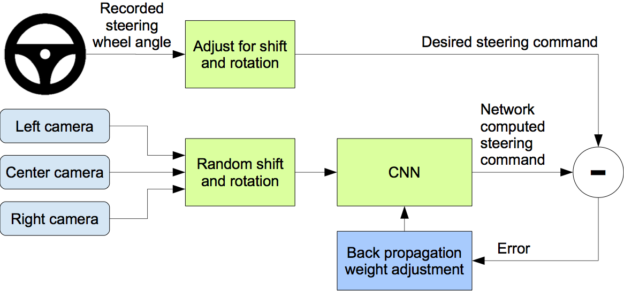
\includegraphics[scale=0.5]{figures/NVIDIA-Training.png}
	\caption{Komponenten des Trainings}
	Quelle: \citeI{NVIDIA-Components}
	\label{img:NVIDIA}
\end{figure}





 Präsentation ALVINN, dann gegenüberstellung mit modernem Netzwerk a la NVIDIA.






Kurzer Blick auf  Self driving car steering angle4 prediction und berkeley (large scale video sets) (vielleicht auchSPÄTER)




Glossar

Convolutional Neural Network CNN



% first example chapter
% @author Jan Robert Rösler 
%
\chapter{Idee}

\section{DroNet und Carolo-Cup}

Die \gls{gl:eth} entwickelte 2018 eine eigene Architektur, mit dem Ziel durch Training auf Fahrbahnbildern eine Drone zu steuern \cite{Loquercio_2018}. 
Das daraus entstandene, von Aufbau und Größe relativ einfach gehaltene Neuronale Netz, war der Anstoß für diese Arbeit. 

Das Netz, siehe Abbildung~\ref{img:DroNet}, bekommt als Input ein 200x200 Pixel großes Bild in Graustufen, der Output ist ein Lenkwinkel und zusätzlich eine Kollisionswahrscheinlichkeit.\\

\begin{figure}[h]
	\centering
	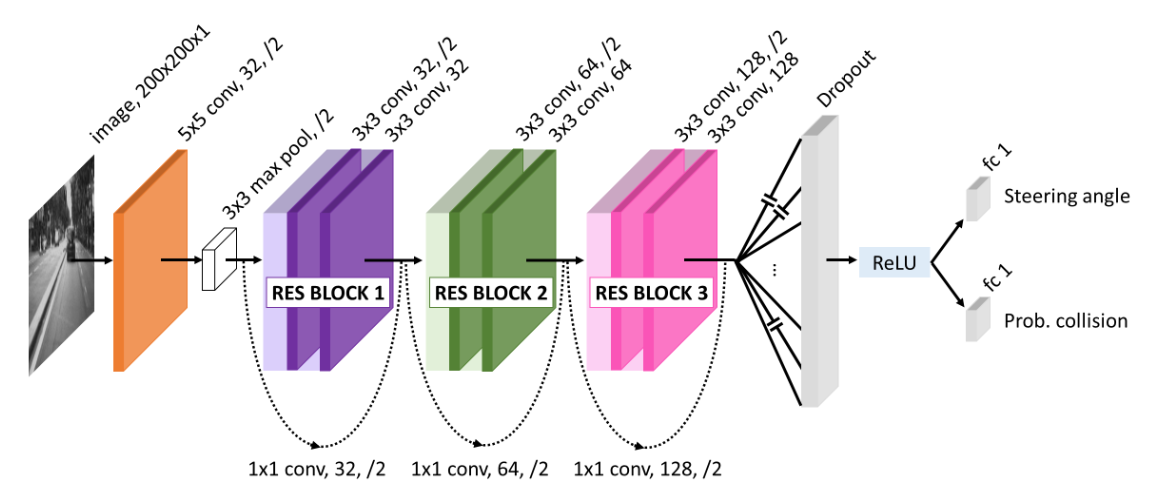
\includegraphics[scale=0.5]{figures/Architecture-DRONET.png}
	\caption{Architektur \textsc{DroNet}}
	\label{img:DroNet}
\end{figure}

Trainiert wurde das Netz auf frei verfügbaren Datensätzen der Firma \gls{gl:udacity}, bestehend aus Bildern aufgenommen mit Kameras hinter der Windschutzscheibe eines Autos bei stundenlagen Fahrten über Amerikanische Highways. Die Aufnahmen sind mit Fahrdaten verbunden, Zeitstempel, GPS-Daten, Beschleunigungswerte und Lenkwinkel wurden für jedes Bild der Aufnahmen gespeichtert. Für das Training von \textsc{\gls{gl:dronet}} werden nur die Bilder der Mittelkamera und der jeweilige Lenkwinkel genutzt.\\
Zusätzlich hat das Team der ETH Zürich eigene Aufnahmen mithilfe einer am einem Fahrrad montierten Kamera im Straßenverkehr gemacht und diese Aufnahmen manuell mit einer Kollisionswahrscheinlichkeit versehen. Wie bereits erwähnt hat das Netzwerk dementsprechend zwei verschiedene Outputs.\\
Für diese Arbeit ist aber nur der Lenkwinkel von Interesse, Kollision spielt als Szenario keine Rolle. Im Entwurf werden dementsprechend Anpassungen gemacht.

Es stellte sich heraus, dass das Modell hervorragend generalisierte und eine Drohne sicher durch ein Straßenszenario steuern konnte, wobei das Szenario sich deutlich von den gelernten Unterschied. Diese Eigenschaft von \textsc{DroNet} möchte ich mir im folgenden zu Nutze machen und auf dieser Basis ein Steuerungsmodell für ein RC-Fahrzeug entwickeln.\\

Die \gls{gl:haw} nimmt bereits seit einigen Jahren am \glqq \gls{gl:carolo} \grqq{} teil, einem Wettbewerb der Technischen Universität Braunschweig. Hier treten Teams einiger deutscher Hochschulen mit RC-Fahrzeugen (Maßstab 1:10) in verschiedenen Disziplinen des autonomen Fahrens gegeneinander an. Der Wettbewerb findet jährlich in Braunschweig auf einem vorbereiteten Kurs statt.
Eine hauptsächlich von den HAW Studenten Nils Schönherr und Gunnar Wolfram aufgebaute Plattform, zu sehen in Abbildung~\ref{img:Carolo-Fahrzeug}, dient dieser Arbeit als Testplattform.

\begin{figure}[h]
	\centering
	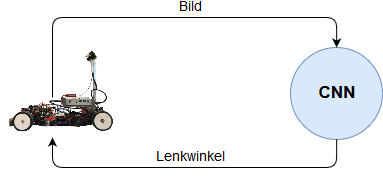
\includegraphics[scale=0.7]{figures/Aufbau.png}
	\caption{Einfacher schematischer Aufbau }
	\label{img:Aufbau}
\end{figure}


Zum entwickeln der Fahrzeuge steht an der HAW eine Teststrecke zur Verfügung, verschiedene Fahrzeugplattformen sind in der Entwicklung.\\
Das Ziel dieser Bachelorarbeit ist, an einem konkreten Anwendungsfall zu zeigen, dass ein Fahrzeug autonom einen Streckenkurs abfahren kann, indem ein neuronales Netz live Bilder der Strecke auswertet und Lenkinformationen für das Fahrzeug berechnet, schematisch dargestellt in Abbildung~(\ref{img:Aufbau}). Da aktive Teams der HAW im Carolo-Cup aktuell klassische (Bildbasierte-) Navigationsansätze verfolgen (Kapitel~\ref{sec:Autonome Navigation mit Bilddaten}), soll die Arbeit auch zeigen, wie eine nächste Generation der Fahralgorithmen für den Carolo-Cup aussehen kann.\\

Die autonome Fahrleistung auf der Teststrecke ist das Hauptaugenmerk, sie zu messen ist zu analysieren ist Bestandteil der Arbeit.




% first example chapter
% @author Jan Robert Rösler 
%
\chapter{Entwurf}


Änderungen an der Architekrtur des Netzes
Lernarchitekrur (Pipepline)
Steuerungsarchitektur
Bilder mit Steuerdaten (Verarbeitungspipelone)
Fahrzeug (Kamera, Rechner etc.)
Strecke 
Training 
Performance (Rechenzeit) bei prediction auf dem Fahrzeug
Kommunikation zwischen C und pYthon
% first example chapter
% @author Jan Robert Rösler 
%
\chapter{Szenarien}


1. Auto mit Dronet 
2. Auto mit adaptiertem Netz
3. Auswertung von Bildern zum beripsiel aus dem Netz (zeigen dass "Kurven" features erlent wurden
% first example chapter
% @author Jan Robert Rösler 
%
\chapter{Auswertung und Zusammenfassung}


\note{Hier werden die Szenarien ausgewertet, miuteinander verglichen und verschiedene Metriken in Tabellen angeben}

MAchbarkeit gezeigt, Optimierungsmöglichkeinte aufzeigen
\input{chapters/7-Resümee}

\cite{chollet2018deep}
\cite{Goodfellow-et-al-2016}


%\bibliographystyle{plain}
\bibliographystyle{dinat}
\bibliography{literature}

% Appendix
\appendix
% !TEX root = ../thesis.tex
% appendix example chapter
% @author Thomas Lehmann
%
\chapter{Anhang}


\IGlossary

\Istatement

\end{document}
